\chapter{Implementation and Testing}\label{Ch5}
In this chapter, the detailed design of the Body Temperature Measuring Wristband from the previous chapter will be implemented and tested. This will be done by firstly designing a Printed Circuit Board (PCB) in CAD software. After the PCB is designed and physically constructed, it will be populated with all the required components. Then the testing phase will begin, where each aspect of the Body Temperature Measuring Wristband will be tested to confirm the expected working of the device.

\section{Implementation}
In this section, the layout and design of the PCB of the Body Temperature Monitoring Wristband will be given. Since the size of the device must be kept as small as possible, the overall footprint of the PCB must also be kept to a minimum. 2D models of the PCB will be given, as well as a 3D model to see how the designed PCB will look like. This section will also show the manufactured and populated PCB of the device. 

\subsection{Printed Circuit Board Design}
The device will have a two-layer PCB, allowing components to either be on the top or the bottom layer. The temperature sensor and related components are on the bottom layer to ensure that it is always in contact with the skin of the user, whilst the other components such as the microcontroller, display, power source, etc. are on the top layer. The software representation of the top 2D view, the bottom 2D view, as well as the combined 2D view of the PCB is shown in \autoref{PCB-Top}, \autoref{PCB-Bottom} and \autoref{PCB-Comb} respectively.
\begin{figure}[H]
	\centering
	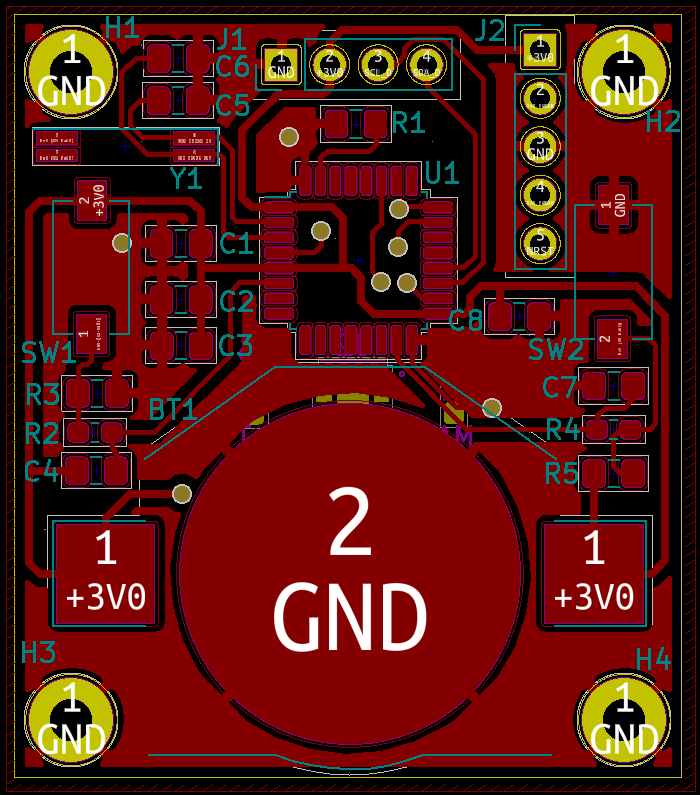
\includegraphics[scale=0.4]{img/PCB-Top.PNG}
	\caption{Software PCB: 2D Top View}
	\label{PCB-Top}
\end{figure}
\begin{figure}[H]
	\centering
	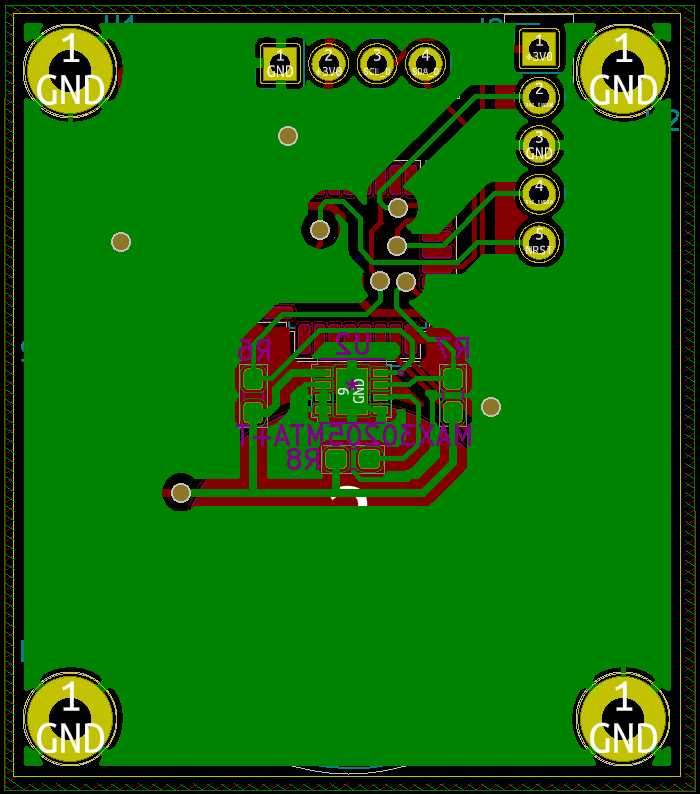
\includegraphics[scale=0.4]{img/PCB-Bottom.PNG}
	\caption{Software PCB: 2D Bottom View}
	\label{PCB-Bottom}
\end{figure}
\begin{figure}[H]
	\centering
	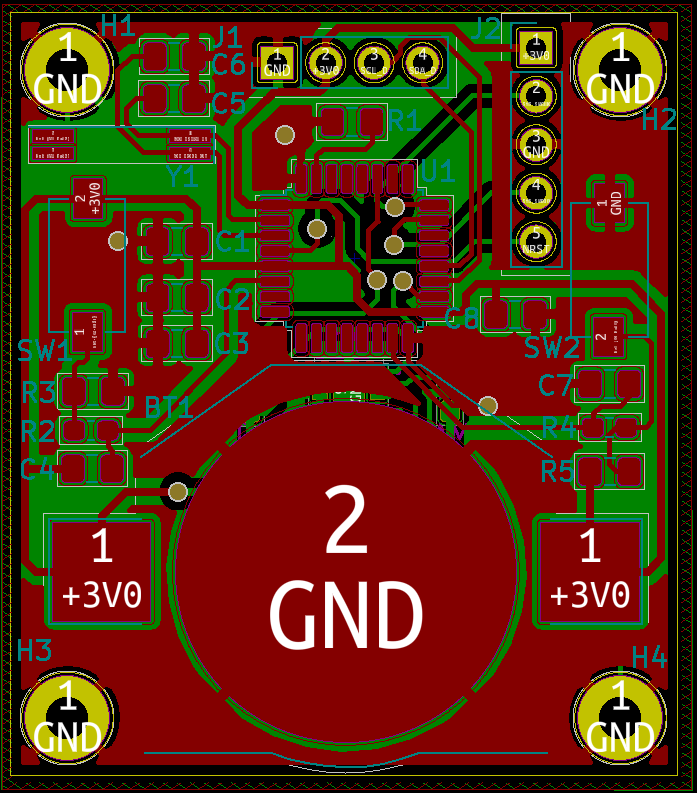
\includegraphics[scale=0.4]{img/PCB-Comp.PNG}
	\caption{Software PCB: 2D Combined View}
	\label{PCB-Comb}
\end{figure}
\noindent
In order to get a better understanding on how the PCB will look like, a 3D rendering of the PCB with all the components populated is shown in \autoref{PCB-3D}.
\begin{figure}[H]
	\centering
	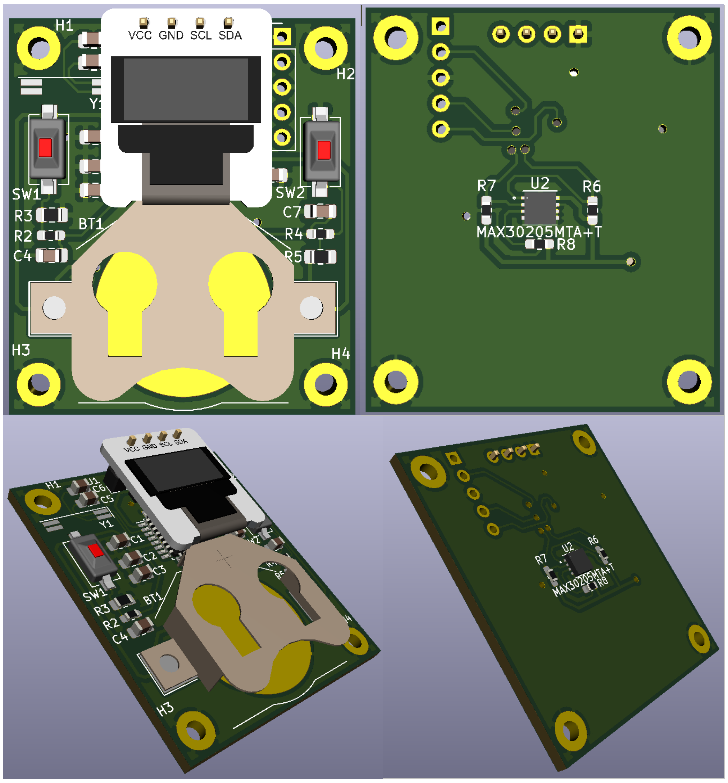
\includegraphics[scale=0.8]{img/PCB-3D.PNG}
	\caption{Software PCB: 3D View}
	\label{PCB-3D}
\end{figure}
\noindent
The dimensions of the designed PCB are shown in \autoref{PCB-Dim}. From this figure, as well as the previous figures showing the PCB layout, it can be seen that the overall footprint of the PCB was kept as small as possible by spacing the components as compactly as the design tolerances would allow. Surface mount components were used where possible and available since through-hole components generally have a larger footprint than that of surface mount components.
\begin{figure}[H]
	\centering
	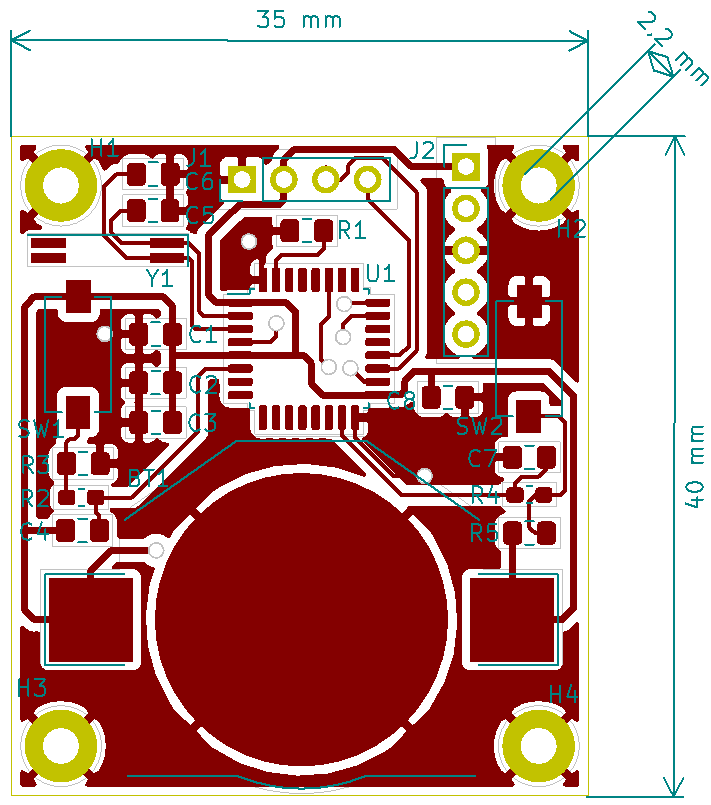
\includegraphics[scale=0.4]{img/PCB-Dim.PNG}
	\caption{PCB: Dimensions}
	\label{PCB-Dim}
\end{figure}

\subsection{Manufactured Prototype Printed Circuit Board}
The manufactured prototype PCB that is populated with the components is shown in this subsection. The top view of the manufactured PCB is shown in \autoref{MPCB-Top} and the bottom view of the PCB is shown in \autoref{MPCB-Bottom}. The testing of the device will be discussed in a later section of this chapter.
\begin{figure}[H]
	\centering
	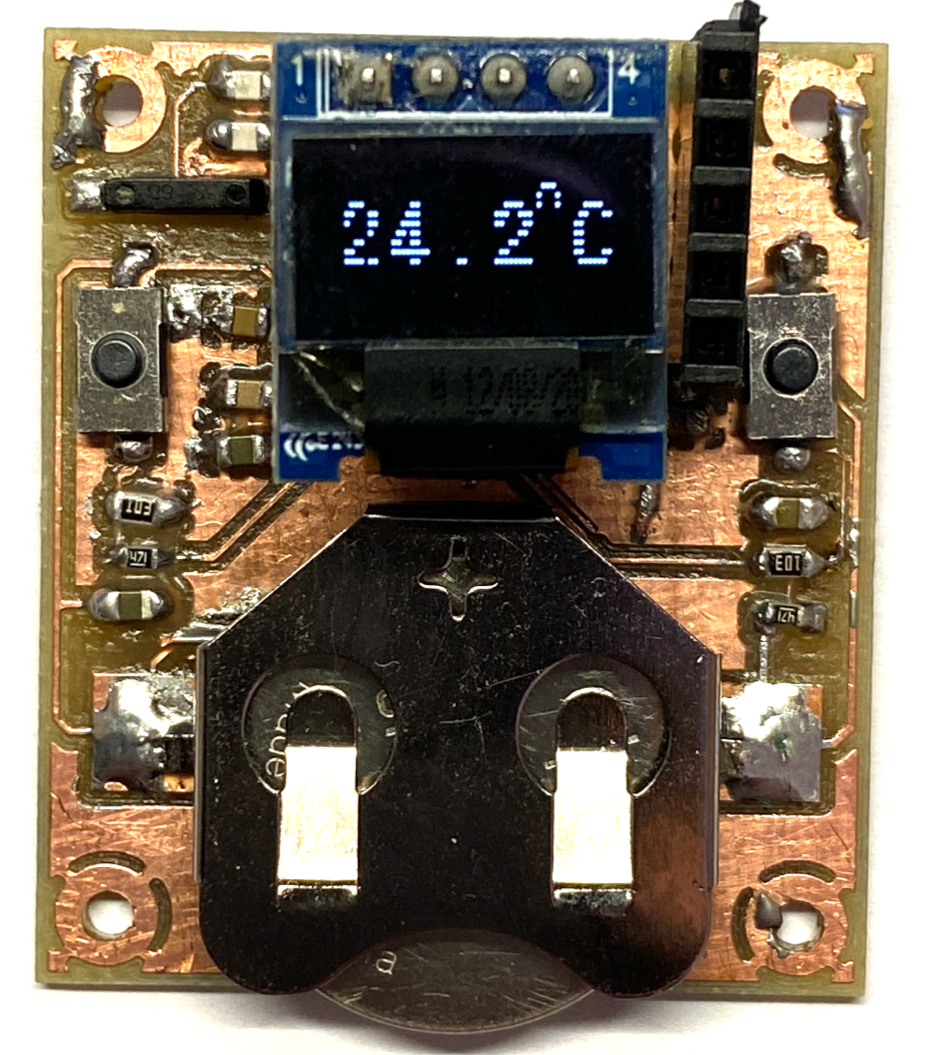
\includegraphics[scale=0.3]{img/MPCB-Top.PNG}
	\caption{Manufactured PCB: Top View}
	\label{MPCB-Top}
\end{figure}
\begin{figure}[H]
	\centering
	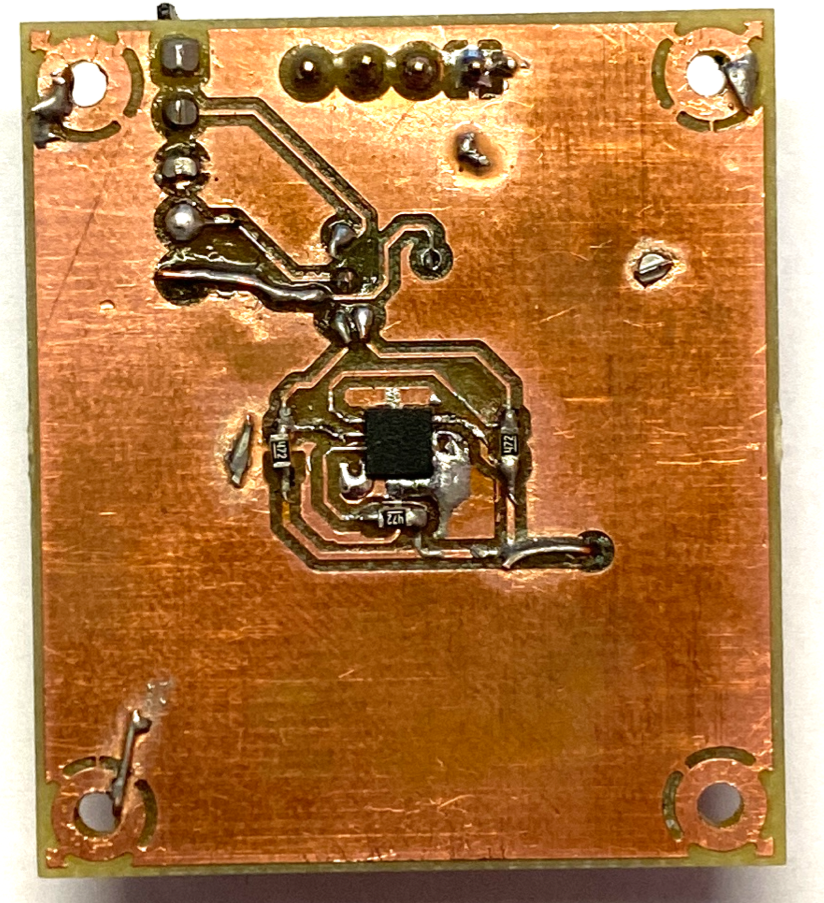
\includegraphics[scale=0.3]{img/MPCB-Bottom.PNG}
	\caption{Manufactured PCB: Bottom View}
	\label{MPCB-Bottom}
\end{figure}

\subsection{Statistical Estimation Model}\label{estm}
In this section, the technique to estimate core body temperature from skin temperature will be discussed. In \autoref{technique} of this report, the statistical estimation is selected as the best technique for this purpose. The method to build the statistical model is explained in \autoref{stat} of this report. The statistical model that will be used for this device is based on that developed by Kwak et al. \cite{Kwak2019} in 2019. In this study, a large amount of data is collected by measuring the skin temperature, the ambient temperature, and the corresponding body temperature to use as a reference in the statistical model. Kwak et al. made the statistic model by collecting data from four students (two men and two women) from May to August 2018 \cite{Kwak2019}. Kwak et al. then derived the relationship between body temperature and skin temperature using the collected data and the method that is described in \autoref{stat} of this report. 
\\
\\
The derived relationship is \cite{Kwak2019}:
\begin{equation}
    Y = 0.109X + 33.07
    \label{estimate}
\end{equation}
\noindent
This relationship are implemented in the firmware to estimate the user's body temperature ($ Y $) from the skin temperature measured by the device ($ X $).

\section{Testing and Results}
In this section, the developed Body Temperature Monitor is tested and results are shown where applicable. 

\subsection{Flash Connector}
The goal of this test is to determine if the STM32 microcontroller of the device can communicate with the ST-LINK/V2-1. This is done in order to verify that the program code can be successfully flashed onto the device. STM developed a tool named STM32 ST-LINK Utility specifically for this reason. This tool will be used to test if communication is possible. \autoref{STLink} shows the result of this test. 
\begin{figure}[H]
	\centering
	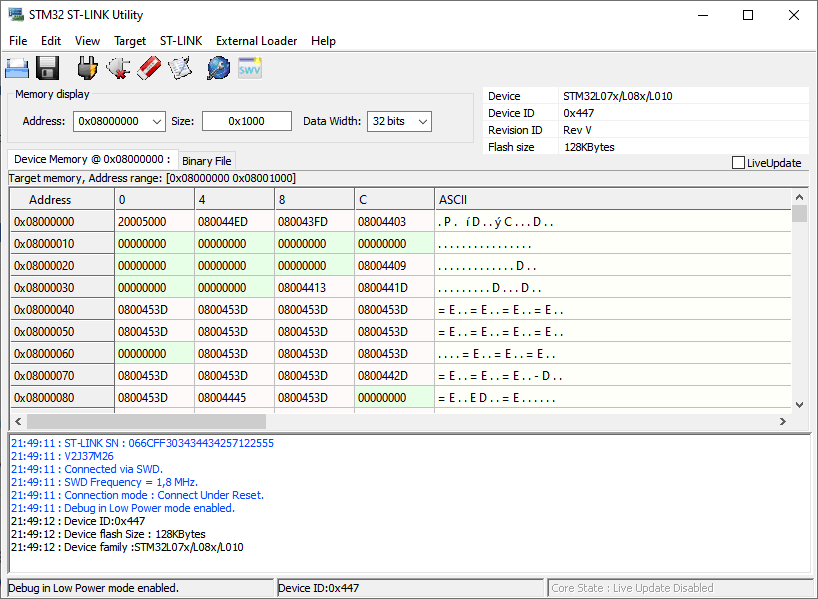
\includegraphics[scale=0.7]{img/STLink.png}
	\caption{STM32 Flash Connection Test}
	\label{STLink}
\end{figure}
\noindent
From the figure above it can be seen that the ST-LINK can successfully connect to the microcontroller of the device through SWD. 

\subsection{Measurement of Skin Temperature}
In this subsection, the accuracy of the measured skin temperature will be determined. Hence, it will be determined how accurate the Body Temperature Measuring device can measure skin temperature compared to a known reference measurement. During this experiment, \autoref{estimate} is not applied in the firmware of the device, resulting in just the measured skin temperature being displayed by the device. To measure the reference temperature (the correct temperature), a Type K thermocouple strapped to the wrist of the user, is used. The Body Temperature Measuring device is then also strapped to the wrist of the user, next to the thermocouple. The error between the two measurements is taken as the absolute difference between the reference temperature and the measured temperature by the device, and the accuracy of the measurement is determined with \autoref{acc}.
\begin{equation}
    Accuracy = 100\% - ((\frac{|Measured - Reference|}{Reference})*100)
    \label{acc}
\end{equation}
\noindent
A few measurements are made during the course of one day, with the method as explained above. The full data-set of the measurements can be found in \autoref{Exp-Data}. \autoref{skin-temp} shows a graph of the reference temperatures versus the measured temperatures. 
\begin{figure}[H]
	\centering
	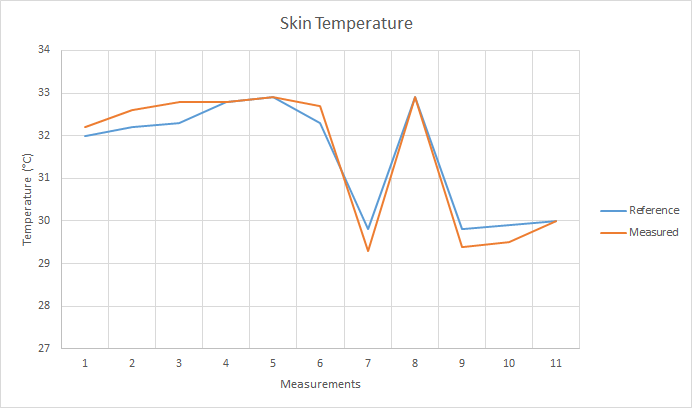
\includegraphics[scale=0.7]{img/Skin-Temp.png}
	\caption{Measurement of Skin Temperature}
	\label{skin-temp}
\end{figure}
\noindent
From \autoref{skin-temp} it can be seen that the temperature measured by the Body Temperature Measuring device varies as the skin temperature varies. The largest absolute difference between the reference temperature and the measured temperature is determined as $ 0.5^{\circ} C $, and the smallest absolute difference is $ 0^{\circ} C $. These absolute errors then relates to a $ 98.32 \%$ measurement accuracy at least, and $ 100 \% $ measurement accuracy at best, for the measurement of skin temperature. 

\subsection{Measurement of Body Temperature}\label{MBT}
In this subsection, the accuracy of the measured body temperature will be determined. Hence, the accuracy by which body temperature gets estimated will be determined. During this experiment, \autoref{estimate} is applied in the firmware of the device, in order for the device to estimate the body temperature of the user by measuring the skin temperature. The reference body temperature of the user is measured with a digital thermometer that is placed under the tongue of the user. The Body Temperature Measuring device is then strapped to the wrist of the user. Once again, the error between the two measurements is taken as the absolute difference between the reference temperature and the estimated body temperature obtained from the device. The accuracy of the measurements is determined with \autoref{acc}.
\\
\\
The measurements are made during the course of two days, at random intervals, with the method as explained above. The number of measurements that were made are 22, and the full data-set of the measurements can be found in \autoref{Exp-Data}. The digital thermometer that are used as a reference measures and displays the body temperature of the user within one minute. When the digital thermometer indicates that its measurement is complete, the temperature that is given by the Body Temperature Measuring device is noted and both these results are added to the data-set. \autoref{body-temp} shows a graph of the reference body temperatures versus the estimated body temperatures.
\begin{figure}[H]
	\centering
	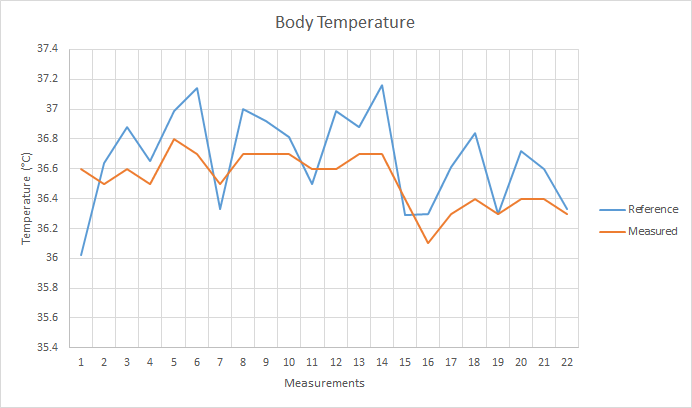
\includegraphics[scale=0.7]{img/Body-Temp.png}
	\caption{Measurement of Body Temperature}
	\label{body-temp}
\end{figure}
\noindent
From \autoref{body-temp} it can be seen that the estimated body temperature relatively varies as the body temperature of the user varies. The largest absolute difference between the reference body temperature and the estimated body temperature is determined as $ 0.58^{\circ} C $. The smallest absolute difference is determined as $ 0^{\circ} C $. These absolute errors then relate to a $ 98.39 \%$ measurement accuracy at least, and $ 100 \% $ measurement accuracy at best, for the estimation of body temperature from the temperature of the skin.

\subsection{Current Consumption of Device}
In this subsection, the current consumption of the device will be determined. This is done to estimate the battery life of the device. The ammeter is series connected into the circuit of the device, and the following measurements are obtained:
\begin{table}[H]
	\centering
	\caption{\textit{Run Mode Current Consumption}}
	\label{tab:8}
	\begin{tabular}{|c|c|}
		\hline
		\textbf{State} &  \textbf{Consumption (mA)} \\
		\hline
		\hline
		Display Temp & 4.49 \\
		\hline
		Display Time & 4.95 \\
		\hline
		Display Date & 5.02\\
		\hline
		Set Hour & 4.72\\
		\hline
		Set Min & 4.71\\
		\hline
		Set Date & 4.68 \\
		\hline
		Set Month & 4.90 \\
		\hline
		Set Year & 5.05 \\
		\hline
		\textbf{AVG} & \textbf{4.815}\\
		\hline
	\end{tabular}
\end{table}
\begin{table}[H]
	\centering
	\caption{\textit{Standby Mode Current Consumption}}
	\label{tab:9}
	\begin{tabular}{|c|c|}
		\hline
		\textbf{State} &  \textbf{Consumption (mA)} \\
		\hline
		\hline
		Standby & 0.01\\
		\hline
	\end{tabular}
\end{table}
\noindent
To estimate the battery life of the device, it is assumed that the user uses the device two times every hour, for 10 seconds. The rest of the time the device will be in standby mode to preserve battery life. An online battery life calculator is used to estimate the battery life. The online calculator is called: Battery Life Calculator for Projects with Sleep Mode, and this calculator includes a 15\% deterioration rate to account for some discharge \cite{Calc2021}. The following were entered into the online calculator:
\begin{itemize}[noitemsep]
    \item Capacity rating of battery (mAh) = 220
    \item Current consumption of device during sleep (mA) = 0.01
    \item Current consumption of device during wake (mA) = 4.815
    \item Number of wakeups per hour (3600 = always ON) = 2
    \item Duration of wake time (ms) = 10000
\end{itemize}
\noindent
The online calculator estimates the battery life of the device as 212.34 days, or 0.58 years, based on the assumptions above. 

\section{Concluding Remarks}
This chapter focused on the implementation and testing of the Body Temperature Monitoring Wristband. Firstly the PCB design of both the top and bottom layers was given, together with a 3D rendered view of the populated PCB. The dimensions of the designed PCB were also given. After this, the manufactured prototype PCB was shown, both the top layer and the bottom layer. In this chapter, the statistical estimation model was also given. The model was based on that developed by Kwak et al. \cite{Kwak2019}, and the relationship between skin temperature and body temperature is given.
\\
\\
After the implementation process was completed, testing began. The communication between the ST-LINK and the STM32 microcontroller of the device was tested, and it was found that communication between the ST-LINK and the microcontroller is possible. This means that firmware can be flashed onto the microcontroller. Next, the accuracy of the device was tested, and the results are shown in \autoref{results}.
\begin{table}[H]
	\centering
	\caption{\textit{Testing Summary}}
	\label{results}
	\begin{tabular}{|c|c|c|}
		\hline
		\textbf{} & \textbf{Skin Temperature} & \textbf{Body Temperature} \\
		\hline
		\hline
		Largest absolute error ($ ^{\circ} C $) & 0.5 & 0.58\\
		\hline
		Smallest absolute error ($ ^{\circ} C $) & 0 & 0\\
		\hline
		Lowest measurement accuracy (\%) & 98.32 & 98.39\\
		\hline
		Highest measurement accuracy (\%) & 100 & 100\\
		\hline
	\end{tabular}
\end{table}
\noindent
The current consumption of the device was also measured, to estimate the battery life of the device. If the device is used two times every hour, for 10 seconds, the estimated battery life of the device is 212.34 days or 0.58 years.

